\documentclass[main.tex]{subfiles}
\begin{document}

\chapter{Theory}
In this chapter the theoretical concepts will be explained.
However it is assumed that the reader has a basic understanding of quantum mechanics.

\section{Superconducting resonators}
Superconducting resonators are used in quantum computing both as the basis for qubits and as readout and control components \cite{}.
Although ideal resonators have equally spaced energy levels, in reality they are more or less anharmonic and the general Hamiltonian for a quantum anharmonic resonator is
\begin{equation}
    \Ham = \omega \au\ad + \frac{\kappa}{2} \qty(\au\ad)^2
    \label{eq:resonator-hamiltonian}
\end{equation}
where \( \omega \) is the resonance frequency, \( \kappa \) is the anharmonic (self-Kerr) term and \(\ad\) is the destruction operator which removes an excitation from the resonator.

The anharmonicity can be vizualised, see \cref{fig:anharmonic-energies}, by plotting the eigenenergies of \cref{eq:resonator-hamiltonian} as a function of \( \kappa \).
A larger (negative) anharmonicity makes the energy spacing smaller for higher excitation states.
This anharmonicity is what permits a resonator to act as a qubit, as it is possible to adress only the \( \ket{0} \) to \( \ket{1} \) level \( \omega_{01} \).

\tikzfig{figs/energy-anharmonic}{The energy levels of a three-level resonator for anharmonicity \(\kappa\in[-0.5,0]\) and \(\omega=1\). Note that the x-axis is reversed.}{fig:anharmonic-energies}{25em}{17em}

\section{Jaynes-Cummings Model}


\section{Visualization of quantum states}
In order to understand the results presented later in this thesis, some visualization techniques of quantum states are shown and explained.

\subsection{Bloch sphere}
\begin{figure}[t]
    \centering
    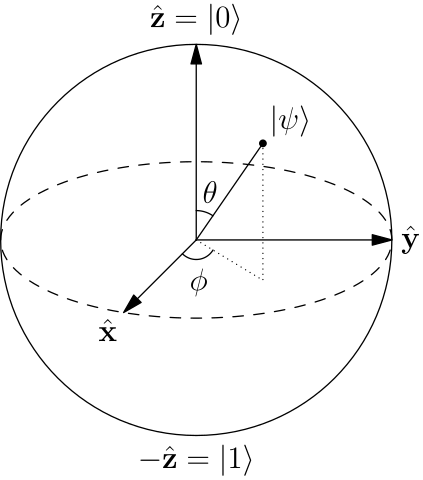
\includegraphics[width=0.3\textwidth]{figs/bloch_sphere.png}
    \caption{Representation of an abritrary pure quantum state on the Bloch sphere.
    \\ Source:~\cite{noauthor_file:bloch_nodate} (CC BY-SA 3.0).
    }%
    \label{fig:bloch_sphere}
\end{figure}

The pure state of a qubit can be visualized on the surface of a unit sphere with the following parametrization
\begin{equation}
    \ket{\psi} = \cos(\frac{\theta}{2})\ket{0} + \ex^{i\phi}\sin(\frac{\theta}{2})\ket{1}
\end{equation}
where \( \theta \) and \( \phi \) are angles which are shown in \cref{fig:bloch_sphere}.
The ground state \(\ket{0}\) is located on the ``north pole'' and the excited state \(\ket{1}\) on the ``south pole''.

% TODO Briefly explain the Bloch sphere representation and give some examples

\subsection{Density matrices and Hinton diagrams}

% TODO Explain the Hinton diagram and density matrix

\subsection{Wigner function}
% TODO Explain why the wigner function is good for visualization.

\section{Bosonic codes}
% TODO Explain what bosonic codes are

\subsection{Cat codes}
% TODO Explain what the cat code basis is and why it can be used for QEC.


\section{Quantum optimal control}
Quantum control is the process of controlling a quantum system by controlling the amplitude of a set of control operators in time~\cite{fisher_optimal_2010}.
Such a system can be described~\cite{fisher_optimal_2010} by a Hamiltonian of the following form
\begin{equation}
    \Ham(t) = \underbrace{\Ham_d}_{\text{Drift}} + \underbrace{u_0(t)\Ham_0 + \dotsc + u_N(t)\Ham_N}_{\text{Control}}.
    \label{eq:optimal-control-hamiltonian}
\end{equation}
The controls are usually electromagnetic pulses changing in time and thus will be referred to as ``pulse shapes''~\cite{fisher_optimal_2010} in this thesis~.

There are two main questions in quantum control: one of \emph{controllability} and one of \emph{optimal control}.
The first deals with the \emph{existence} of solutions given a Hamiltonian and the second with the \emph{optimized} solutions for the pulse shapes \(\qty{u_i(t)}\)~\cite{dalessandro_introduction_2007}.
The optimal solutions are generally not analytically solvable and thus the pulse shapes need to be discretized in time and numerically optimized using algorithms.
The algorithm used for this thesis is called Krotov's method and will be presented in the Method chapter.

\subsection{Unitary transformation}
A unitary transformation can significantly simplify systems that are hard to simulate.
This idea will be conceptually presented here and then implemented in the Method chapter.
The unitary transformation that is used is a special case of transformations called the \emph{interaction picture} where the Hamiltonian is split up into a time-independent and time-dependent part
\begin{equation}
    \Ham(t) = \Ham_A + \Ham_B(t).
\end{equation}
By choosing the unitary operator \( \hat{U} = \ex^{i \Ham_A t} \) the unitary transformation takes us into the interaction picture
\begin{align*}
    \Ham &\rightarrow~ \hat{U}\qty[ \Ham_A  + \Ham_B(t)]\hat{U}^\dagger + i\dv{\hat{U}}{t}\hat{U}^\dagger =\\
    &=~ \hat{U}\Ham_A\hat{U}^\dagger + \hat{U}\Ham_B\hat{U}^\dagger + i\qty(i\Ham_A t)\ex^{i \Ham_A t}\ex^{-i\Ham_A t}=\\
    &=~ \Ham_A + \hat{U}\Ham_B\hat{U}^\dagger - \Ham_A = \hat{U}\Ham_B\hat{U}^\dagger
\end{align*}



\end{document}
